% =====================================================
\chapter{Characterisation of a model}
\label{chap:model_characterisation}

\section{Deadheading problem and the Single Cycle protocol}
\label{sec:existing_summary}

The material handling device proceeding or returning empty while attending to an order is the deadheading problem. By default or following the single cycle protocol,
when travelling to pick the item, the forklift is empty. Also, when travelling back after storing an item, the forklift is empty.

\begin{figure}[!h]
    \centering
    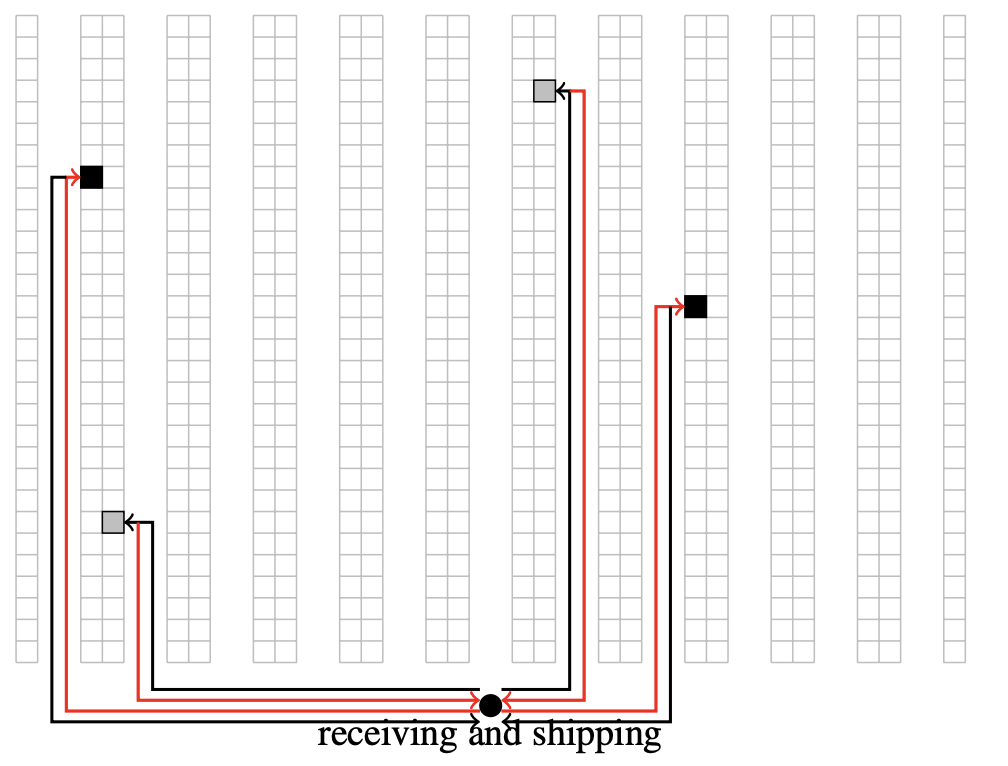
\includegraphics[width=0.65\linewidth]{images/Single_Cycle.png}
    \caption{Single Cycle Protocol}
    \label{fig:single_cycle}
\end{figure}

\section{Dual Cycle Protocol}

Enter, the dual cycle protocol. In the dual cycle protocol, a picking operation is paired with a putting (stowing) operation. This way while returning after the stow operation,
the picker proceeds to the pick operation, thereby never going empty handed.

\begin{figure}[!h]
    \centering
    \includegraphics[width=0.65\linewidth]{images/Dual_Cycle.png}
    \caption{Dual Cycle Protocol}
    \label{fig:dual_cycle}
\end{figure}

The Dual cycle protocol relies on the following optimization model: 

\begin{itemize}
    \item M is set of locations covered by store operations.
    \item N is set of locations covered by picking operations.
    \item $i \in M \text{ and } j \in N$
    \item $d_{ij}$: distance between locations $i$ and $j$
    \item $x_{ij}$: 1 if store operation at $i$ is succeeded by
    pick operation from $j$, 0 otherwise

    \begin{align*}
    \min \quad & \sum_{i,j} d_{ij}x_{ij} \\[0.2cm]
    \text{s.t.} \quad
    & \sum_i x_{ij} = 1 \qquad \forall j \\[0.1cm]
    & \sum_j x_{ij} = 1 \qquad \forall i \\[0.1cm]
    & x_{ij} \in \{0,1\} \qquad \forall i,j
    \end{align*}  
    
\end{itemize}

\paragraph{Summary}

% =====================================================
% \section{Summary}
% \label{sec:existing_summary}

% StyleShot produced aesthetic but non-physical results, CSGO provided structured disentanglement but lacked volumetric realism, and InstantStyle achieved balanced, physically grounded stylization.  
% The tuned-soft InstantStyle run proved most effective, motivating further extensions such as \textbf{InstantStyle-Plus} and \textbf{CSD-Guided Diffusion} for controlled, environment-aware adaptation.
